% !TeX spellcheck = en_GB
\documentclass[10pt]{imeko_acta}

%----------------------------------------------------------------------------------------
% Completed by Authors - Everything below here
%
\PaperTitle{Template for an Acta IMEKO paper} % Article title

\author[1]{Thomas Bruns}
\author[2]{Dirk Röske}
\author[2]{Paul P. L. Regtien}
\author[3]{Francisco Alegria}
\author[1]{Corey Stambaugh}

\affiliation[1]{Physikalisch-Technische Bundesanstalt, Bundesallee 100, 38116 Braunschweig, Germany}
\affiliation[2]{Measurement Science Consultancy, Julia Culpstraat 66, 7558JB Hengelo, The Netherlands}
\affiliation[3]{Instituto de Telecomunicações and Instituto Superior Técnico, Universidade Técnica de Lisboa, Av. Rovisco Pais 1, 1049-001 Lisbon, Portugal}

\CorrespondingAuthorNumber{3}
\CorrespondingAuthorEmail{corey.stambaugh@nist.gov}

% Keywords - if you don't want any simply remove all the text between the curly brackets
\Keywords{Journal; template; IMEKO; Microsoft Word} 

%Leave blank for no funding
\Funding{[Optional, if applicable] This work was supported by Measurement Science Consultancy, The Netherlands.}
%Leave blank for no funding, like this
%\Funding{}

%----------------------------------------------------------------
% Completed by Editors - You can fill in but Editor will finalize
%----------------------------------------------------------------
\Editor{Francesco Lamonaca}
\EditorAffiliation{University of Calabria, Italy}
\Received{January 1, 2021}
\FinalForm{January 31, 2021}
\Published{March 6, 2021}
\VolumeNumber{4}
\VolumeMonth{October}
\VolumeYear{2021}
\IssueNumber{1}
\ArticleNumber{5}
\SubmissionNumber{1676}

%	ABSTRACT - length less than 200 words. 
%---------------------------------------------------------------
\Abstract{The editorial team of Acta IMEKO strongly encourages 
authors to use this \LaTeXe template file to produce their manuscript. 
The abstract should be composed in a way suitable for publication 
in the abstract section of electronic journals, 
and should state concisely what it is written in the paper. 
Important items are the aim of the research, the basic method and the major achievement 
(also numerically, when applicable). The length should not exceed 200 words.
}

%----------------------------------------------------------------------------------------

\begin{document}

\maketitle % Print the title and abstract box
%\VolumeNumber{4}
\section{Introduction}

The introduction describes the background of the research, a 
short review of related research published in recent literature, 
together with the major claims setting the framework of the 
present publication. References should be related to the present 
publication, not just a list of papers merrily showing the authors'
knowledge of the literature. This relation must be made explicit. 
The newly presented method is shortly introduced, as an 
alternative to previously published methods, with mention of the 
advantages aimed at.

To minimize editing by the editorial team, authors are asked 
to follow the styles that go with this template. The font size of 
the body text is 10 pt and the font type is Garamond. For the 
header of a section use the style named “Level1Title”.

The introduction ends with an outline of the remainder of the 
paper, for instance as follows. In Section 2 we will discuss how 
the paper can be divided in sections and subsections, and an 
indication of the use of numbering and heading format is 
outlined. In the next two sections the use of illustrations and 
equations is described. In Section 5 methods for citing references 
are given. Finally, in the concluding section the major rules are 
summarized.\vfill\par

\section{First Page}

The first page should have the title of the paper, the authors names (do not use initials for the first and last name), and the author affiliations.

Following should be an abstract and 3 to 5 keywords separated by a semicolon. The next 4 items (citation, editor, dates and copyright) are to be updated by the editor. The paper information section ends with reference to the funding (leave blank if necessary) and the name and email address of the corresponding author. %The latex template indicates which areas need updated by author and which by the editor. 

The header and footer have information about the publication that is to be updated by the editor. Page numbers appear in the bottom right corner and are updated automatically. 

\section{About Sections}

The body of the paper is divided into sections and, when readability requires it, subsections. This helps the reader to recognize the various elements of the paper, such as background theory, modelling and simulations, experimental setup, experimental results with evaluation, conclusions, references, acknowledgements and, when appropriate, appendices. 

Pages should be laid out using two columns, as done in most journals, to increase readability.

\begin{figure}
	\centering
	
\includegraphics[width=0.68\linewidth]{image1}
	\caption{Stamp issued to help people getting familiar with SI units.}
	\label{fig:image1}
\end{figure}

	

\subsection{Subsections} \label{sec:sub1}

If a section is long or deals with different topics, make a subdivision in subsections. Avoid further subdivision of a subsection. When subsections are used, there must be at least two. Use the style named ``Level2Title'' for the header of a subsection.

\subsection{Numbering of subsections}

Subsection numbering follows the outline numbering format which is configured in the template. Subsection headings use the Calibri font and are in bold.


\begin{figure}[!b]
	\centering
	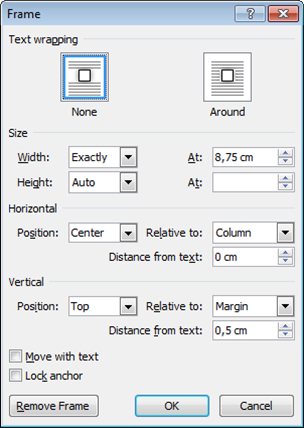
\includegraphics[width=.925\columnwidth]{image2}
	\caption{Microsoft Word frame formatting window. It can be accessed by clicking on the frame content to make the frame border visible, clicking in the frame border to select it and finally right click the frame border to show up the pop-up menu and choosing the option "Format Frame".}
	\label{fig:image2}
\end{figure}

This template uses automatic outlined numbering for the sections and subsections. We recommend that the author makes use of this feature. If the author does not feel comfortable with it, he may choose to manually number the sections and subsections.

Configuring a blank Word document to use automatic outline numbering is not always as straightforward as it should be. We point out, nevertheless, that the configuration is already done in this template and the author just can use it. It suffices to place the cursor in the section or subsection title and select the "Level1Title" or "Level2Title" styles already available from the menu or ribbon. This simple procedure is the same that should be used for all other parts of the paper (paper title, main text, abstract, etc.). The author does not have to worry about the numbering at all.

\begin{figure}[!tb]
	\centering
	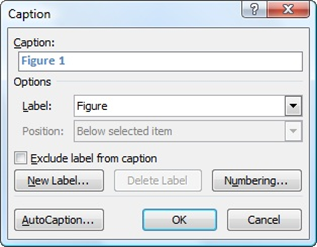
\includegraphics[width=.955\columnwidth]{image3}
	\caption{Microsoft Word caption insertion window. It can be accessed by right clicking on the picture or table and selecting "Insert Caption" from the pop-up menu.}
	\label{fig:image3}
\end{figure}

An even simpler procedure would be just to copy and paste an existing section or subsection title and rewrite the text. The author, however, can choose to use manual numbering by deleting the automatic number that comes with the use of the proper style and input the numbers he wishes for each section.

\section{About Illustrations and Table}

\subsection{Location}

Illustrations and tables can have two formats: column wide or page wide. Figure 1 is an example of the first kind\cite{Fazio1995}. Figure 5 gives an example for a page wide figure.
Page wide figures and tables should be placed inside a frame. Column wide ones can be placed inside a frame or directly in the middle of the body text. In both cases they should be located on top or bottom of the page where they are first referred to in the text if possible. Figures should be configured with the "Figure" style.


\subsection{Managing Frames}

To create a frame, we recommend that the author copies and pastes one of the frames in this template. Before doing that, however, it is important to understand how they are configured. 

\begin{figure*}[!t]
	\centering
	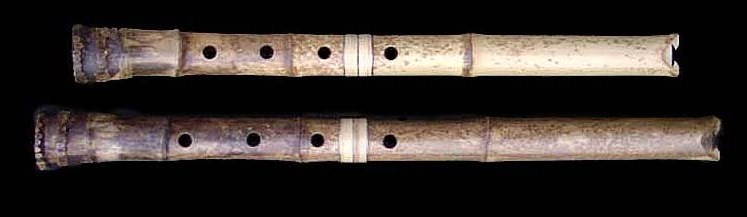
\includegraphics[width=.9\linewidth]{wide_image}
	\caption{Shakuhachi: old Japanese length standard: 1 shaku = 30.3 cm}
	\label{fig:wideimage}
\end{figure*}

Figure 2 shows the window where the configuration is done. It can be accessed by: 
\begin{enumerate}
	\item clicking on the frame content to make the frame border visible;
	\item clicking in the frame border to select it;
	\item right clicking the frame border to show up the pop-up menu and choosing the option "Format Frame".
\end{enumerate}

That window has 4 sections organized from top to bottom ("text wrapping", "size", "horizontal" and "vertical"). 
Text wrapping should always be set to none. The size should be exactly 18 cm for page wide illustrations and tables and 8.75 cm for column wide ones. The horizontal setting should be centred relative to the column or page for column wide or page wide content respectively. The vertical setting can be top relative to margin or bottom relative to margin depending where the frame is supposed to be located (top or bottom) of the page.
The frames in this template have all the proper formatting and can be used as is. The only setting the author will need to manage when crating new frames by copy and pasting existing ones is the vertical setting that will have to be changed from top to bottom depending on the new frame location.

\begin{figure}[!t]
	\centering
	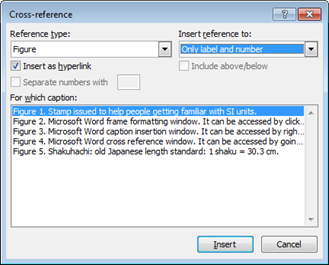
\includegraphics[width=\columnwidth]{image4}
	\caption{Microsoft Word cross reference window. It can be accessed by going to the menu "References" and choosing "Insert Cross Reference".}
	\label{fig:image4}
\end{figure}







The copying and pasting of frames should be done with care because the new frame will have the same configuration as the original frame and may overlap with it making one of them invisible to the user. We suggest that the author selects the original frame, chose "copy" (CTRL+C), place the cursor in a page or column that has no frame in the same position as the original and chose "paste" (CTRL+V). It is up to the author to manage in which page or column each frame is to be located.

The more complicated situation is when the author wants to copy a page wide frame that is in the top of a page to a new frame located in the bottom of the same page. Because the original frame vertical setting is top the new pasted frame will also have the same setting and will overlap with the original one if placed in the same page. The solution is to paste the frame in a different page where no frames exist in the top (can be a temporary blank page at the end of the document), change the vertical setting to bottom and perform a cut and paste to the desired page. It will then show up at the bottom of that page.
If the author prefers to create a frame from scratch, he/she can choose "insert text box". Then he/she should right click on the text box border and select from the pop-up menu the option to format the text box. In the window that becomes visible press "convert to frame". The properties of the frame should be adjusted as described previously.




\subsection{Captions}

Place the figure captions directly below the figure inside the frame and choose the style “Figure caption”. Figure captions have the format “Figure x. aaa.” where x stands for the figure number and aaa for the figure caption. Figures should be numbered consecutively with Arabic numerals starting from 1. Note that the caption should end with a period. 

The paragraph spacing before the caption should be 6 pt and after the caption should be 12 pt. This is defined in the “Figure caption” style. This formatting should be overridden in the case of figures placed at the bottom of a page so that the paragraph spacing after the caption is 0. See, for instance, the caption of Figure 5.

Table captions should be placed inside the frame directly above the table. Format it with the style “Table caption”. Table captions have the format “Table y. aaa.” where y stands for the table number and aaa for the table caption. Tables should be numbered consecutively with Arabic numerals starting from 1. Tables and figures should have separate numberings. Note that table captions should also end with a period. 

The paragraph spacing before the table caption should be 12 pt and after the caption should be 6 pt. This is defined in the “Table caption” style. This formatting should be overridden in the case of tables placed at the top of a page so that the paragraph spacing before the caption is 0. See, for instance, the caption of Table 1.


\subsection{Tables}

Tables span a full page in width, for example, Table \ref{tab:tab1}, or a full column, see Table \ref{tab:tab2}. Avoid breaking tables across pages.
Table captions are placed ABOVE the table. 
Table 1 summarizing the various styles used in this template, whereas Table 2 shows a subset of the data given in Table 1.

\begin{table*}[!h]
	\caption{Overview of styles and font sizes used in this template.}
	\label{tab:tab1}
	\centering
	\renewcommand{\arraystretch}{1.15}\footnotesize
	\begin{tabularx}{\textwidth}{lCCCC}
		\toprule
		Section & Font & Size (pt) & Format & Special \\
		\midrule
		Title & Calibri & 20 & bold & Only first letter is capital \\
		Authors & Calibri & 12 & bold &  \\
		Affiliation and email address & Calibri & 9 & italic &  \\
		Abstract text & Calibri & 9 & normal &  \\
		Keywords & Calibri & 8 & normal & label in bold \\
		Citation & Calibri & 8 & normal & label in bold \\
		Editor & Calibri & 8 & normal & label in bold \\
		Dates & Calibri & 8 & normal & label in bold \\
		Copyright & Calibri & 8 & normal & label in bold \\
		Funding & Calibri & 8 & normal & label in bold \\
		Corresponding author & Calibri & 8 & normal & label in bold \\
		First-level Section headings  & Calibri & 10 & Bold & numbered, all caps \\
		Subsection headings & Calibri & 9 & Bold & outline numbered \\
		Body text & Garamond & 10 & normal & justified \\
		Acknowledgements, Appendix & Garamond & 10 & normal & as body text \\
		Footnotes  & Calibri & 8 & normal & as body text \\
		Equations & Garamond/Symbol & 10 & italic & numbered \\
		Equations (subscript/superscript) & Garamond/Symbol & 70\% of 10 & italic & numbered \\
		Equations (sub-subscript/superscript) & Garamond/Symbol & 60\% of 10 & italic & numbered \\
		Table text & Calibri & 8 & normal & bold headings \\
		Figures & Calibri & 9 & normal & centered \\
		Captions of figures and tables & Calibri & 8 & normal & justified \\
		References & Garamond & 9 & normal & numbered \\
		\bottomrule
	\end{tabularx}
\end{table*}

\begin{table}[!b]
	\caption{Example of a small table.}
	\label{tab:tab2}
	\centering
\begin{tabularx}{\columnwidth}{lC}
	\toprule
	Section & Font \\
	\midrule
	Title & Calibri \\
	Authors & Calibri \\
	Affiliation and email address & Calibri \\
	Abstract text & Calibri \\
	Keywords & Calibri \\
	Citation & Calibri \\
	Editor & Calibri \\
	Dates & Calibri \\
	Copyright & Calibri \\
	Funding & Calibri \\
	Corresponding author & Calibri \\
	First-level Section headings  & Calibri \\
	Subsection headings & Calibri \\
	\bottomrule
\end{tabularx}
\end{table}

\subsection{Numbering}

Microsoft Word permits to have figure and table numbering done automatically. The author is asked to use this feature, if possible, instead of numbering them by hand. The captions in this template already use automatic numbering. The best way for the author is just to copy and paste those captions and change the text accordingly. Because the number in the copied caption label will not be automatically updated, the author can place the cursor in the caption number and press the key F9 to update it (the number background turns grey because it is a "field code").

If the author wants to use automatic caption numbering but creates captions from scratch, he/she can right click on the picture or table and select "Insert Caption" from the pop-up menu. A window will be displayed (Figure 3) where one can choose the label "Figure" or "Table" and insert the caption text. If those labels are not in the drop-down list the author can add them by using the "New Label" button.


\subsection{Referring to figures and tables in the text}\label{sec:reffig}

If automatic caption numbering is used the author should refer to the figures and tables in the text using automated references. A reference can be inserted in a given point in the text by going to the menu "References" and choosing "Insert Cross Reference" (Figure 4). Select which figure or table are to be cited, the label type ("Figure" or "Table") and that only the label and number should be used in the citation. Keep the option "insert as hyperlink". 

\section{About Equations}

All equations should be numbered consecutively throughout the paper. Do not use outline numbering per section. \LaTeXe\ automatically handles all of this. Numbers are placed between parentheses aligned right, and without a label, see equation (\ref{eq:eq1}) as an example, expressing the saturation current ID in a MOSFET transistor \cite{Middelhoek1989}:

\begin{equation}\label{eq:eq1}
I_D = \frac{W \mu \epsilon_0 \epsilon_{0x} V^2_{GS}}{2Lt}
\end{equation}

where $W$ is the channel width, $L$ the channel length, $\epsilon_0$ the dielectric constant of free space and $\epsilon_{0x}$ of the oxide, $\mu$ is the mobility in the channel, $t$ the oxide thickness and $V_{GS}$ the gate voltage \cite{Middelhoek1989}. Make sure that all symbols are defined unambiguously. When confusion may arise, add the units of the parameters between square brackets. Use SI and derived units only \cite{Grattan1994}. 

Long equations that normally span more than one column should be wrapped over more lines, broken at a suitable place by arithmetic symbols ($=$, $+$, $-$, $\times$) as separator. An example is equation  (\ref{eq:eq2}) about the surface heat flux per unit area along a flat plate \cite{Lighthill1950}.

\begin{multline}\label{eq:eq2}
P^{"}_f(x) = 0.538\kappa_f \left(\frac{Pr}{\nu}\right)^{1/3}\left(\frac{\tau_w(x)}{\mu}\right)^{1/2} \times \\
\int_{0}^{x} \left(\int_{0}^{x}\sqrt{\frac{\tau_w{zeta}}{\mu}d\zeta} \right)^{-1/3} \frac{\partial T_w(x_1)}{\partial x_1}dx_1
\end{multline}

Equations are considered part of the previous sentence and should, when appropriate, have a period or a comma after them, as in (2).

Note that punctuation of equations must follow the normal rules of grammar. Therefore, for example, equations can be followed by a dot only if the sentence is finished.

Very short equations that are not further referred to may be inserted in line with the text, for instance $R = V/I$. Make sure that all variables are in italic, also when used in the main body. 

Note that the font size for equations is 10 pt and that it must be reduced to 70 \% and 60 \% in the case of subscript/ superscript and sub-subscript/superscript respectively.

Mind proper notations. Some typical errors or wrong formats 
should be avoided at the very beginning: 
\begin{itemize}
	\item variables must be italic: V2
	\item numbers and units not: 3 V
	\item space between value and unit: 3 kHz, 10 %, 5 °C
	\item units never between square brackets [...].
\end{itemize}

\section{About references and citations}

References are limited to published works or papers that have been accepted for publication and should give full bibliographical information. They are placed in the section References at the end of the manuscript, in order of their appearance in the text.

References are cited in the text by a number between square brackets. Ensure that every reference cited in the text is also present in the reference list and vice versa.

Citation of multiple or consecutive references must follow the notation [1], [2], [4] or [1]-[3], respectively.

Unpublished results and personal communications may be included in the reference section following the standard reference style and should include a substitution of the publication date with either "Unpublished results" or "Personal communication". 

Citation of a reference as "in press" implies that the item has been accepted for publication.
The format of references is as follows:

\begin{enumerate-a}
	\item For journal articles: Initials and last name(s) of each author, Title of article (first word only capitalized), Journal title, volume number, (year), pages.
	\item Book references: Author(s) as above, Title of book (main words capitalized), publisher, city of publication, year, ISBN. 
	\item For a chapter in an edited book: Author(s) as above, Title of article (first word only capitalized), in: Title of book (main words capitalized). Editor(s). Publisher, city of publication, year, ISBN, pages.
	\item Conference proceedings: Initials and last names of each author, Title of article (first word only capitalized), name of the conference, place, country, date, pages.
	\item Links to web content, for example freely downloadable papers, can be included as shown in [5].
	\item Where available, DOIs of references must be added as shown in [1].
	\item References that are not in English, must be followed by the language, for example, in the form [In Italian] as shown in [7].
\end{enumerate-a}

There is a section break at the end of the paper (after the references) so that the content of the last page is equally divided between the two columns.


\section{conclusions}
The concluding section contains the major achievements of the research presented in the manuscript. It should be concise but informative\cite{cruz2008}. When numerical results are an essential part of the research, for instance a wider measurement range, higher uncertainty \cite{Pop2006}, they should be included in the conclusions.
Notice that conclusions are not the same as an abstract.


\section*{acknowledgment} 

Here persons or institutes may be acknowledged for their technical, scientific or financial support. List them in this section, and not as a footnote or otherwise.

\bibliographystyle{imeko_acta}
\bibliography{imeko_acta.bib}

\end{document} 
